\documentclass[12pt]{article}
\usepackage{graphicx}
\usepackage{amsmath}
\usepackage{amssymb}
\usepackage{latexsym}
%\usepackage{epsfig,enumerate,amsmath,amsfonts,amssymb,setspace}
\usepackage{indentfirst}
\usepackage{epsfig,float}
\usepackage{wrapfig,lipsum}
\usepackage{mathrsfs}
\usepackage{algorithm}
\usepackage{algorithmic}
\usepackage[algo2e,ruled,vlined]{algorithm2e}

\newtheorem{definition}{Definition}[section]
\newtheorem{theorem}{Theorem}[section]
\newtheorem{lemma}{Lemma}[section]
\newtheorem{corollary}{Corollary}[section]
\newtheorem{proposition}{Proposition}[section]
\newtheorem{obs}{Observation}[section]
\newtheorem{claim}{Claim}[section]
\newtheorem{res}{Result}[section]
%\newtheorem{algorithm}{Algorithm}[section]
\newcommand{\proof}{{\bf Proof : }}
\usepackage{graphicx}
\setlength{\textheight} {9. in} \setlength{\textwidth} {6.3 in}
\voffset -1 in \hoffset -0.5 in \topmargin .8 in
\setlength{\evensidemargin} {0.6 in} \setlength{\oddsidemargin}{0.6
in} \setlength {\columnsep}{6 mm} \baselineskip 8 mm


%\journal{Discrete Applied Mathematics}

\begin{document}

%\begin{frontmatter}

%% Title, authors and addresses

%% use the tnoteref command within \title for footnotes;
%% use the tnotetext command for theassociated footnote;
%% use the fnref command within \author or \address for footnotes;
%% use the fntext command for theassociated footnote;
%% use the corref command within \author for corresponding author footnotes;
%% use the cortext command for theassociated footnote;
%% use the ead command for the email address,
%% and the form \ead[url] for the home page:
%% \title{Title\tnoteref{label1}}
%% \tnotetext[label1]{}
%% \author{Name\corref{cor1}\fnref{label2}}
%% \ead{email address}
%% \ead[url]{home page}
%% \fntext[label2]{}
%% \cortext[cor1]{}
%% \address{Address\fnref{label3}}
%% \fntext[label3]{}

\title{Stock Price Prediction Using Text Analysis}


\author {Ankit Panda, Abhinandan Bhatnagar, 
Aman Mittal, Nikhil Mahipal\\ Rahul Garg, Rishabh Bansal  \\ \\
Department of Computer Science and Engineering\\
Bennett University, Greater Naoida, UP}
%% use optional labels to link authors explicitly to addresses:
%% \author[label1,label2]{}
%% \address[label1]{}
%% \address[label2]{}
\date{}
\maketitle

%\author{Ankit Panda}
%\ead{ankit.panda@bennett.edu.in}
%\cortext[cor1]{Corresponding Author}

%\address{Department of
%Computer Science and Engineering, Bennett University, Greater Noida , INDIA}

%\end{frontmatter}

\section{Experimental Results}
For the Stock Prediction we have used google's Colaboratory, it is a jupyter notebook environment that runs entirely in the cloud, this aids our systems in heavy processing power.
\ \
The data that we fetch are of two kinds: The Numerical data and the corresponding news articles for the particular stock. The following shows the fetching of the articles.
\ \
\begin{center}
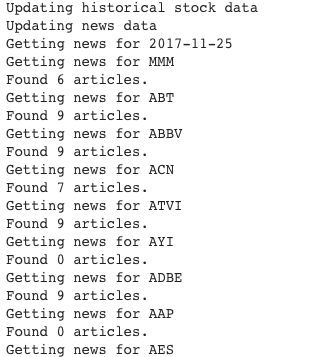
\includegraphics[width=0.6\textwidth]{Getting_articles.png}
\end{center}
\\
The following piece of code fetches the data for us i.e. the Historical data for the stocks. 
\\
\begin{center}
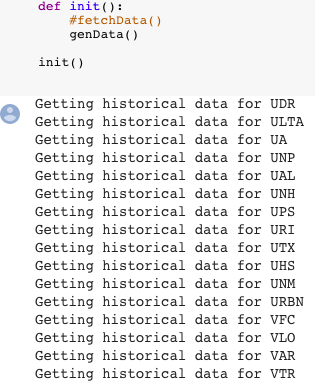
\includegraphics[width=0.5\textwidth]{Getting_HSD.png}
\end{center}
\\
The Historical data and the articles are then stored date wise for a total of 1 year ranging from 27th Nov 2017 to 23 Nov 2018. The Following is an example of the APPL stock info for the past one year. The dataframe contains: open, high, low, close & volume.
\begin{left}
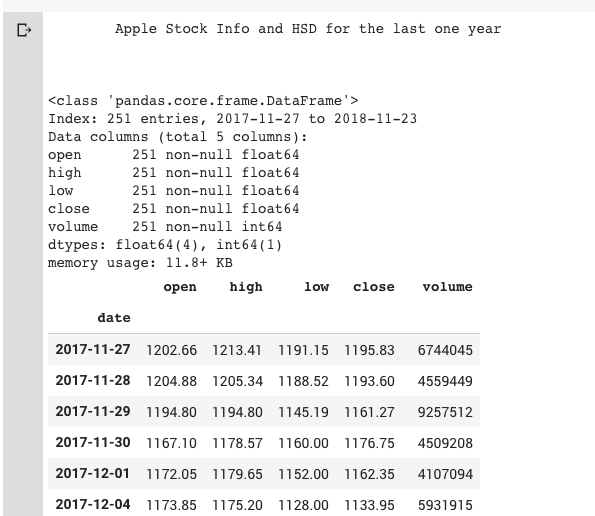
\includegraphics[width=0.4\textwidth]{Stock_dataf.png}
\end{left}
\begin{right}
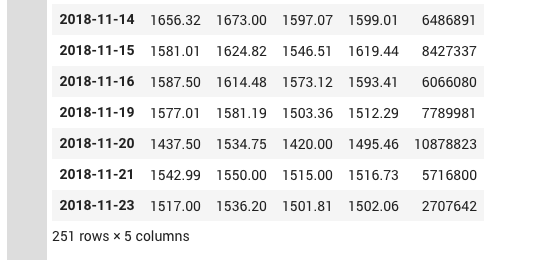
\includegraphics[width=0.7\textwidth]{Stock_dataf2.png}
\end{right}
\\

\\
After Collecting all the prerequisite data for processing we use the Function Gendata to produce the Sentiment analysis of the article, Subjectivity of the Article, opening price of the Stock and finally the opening price of the stock after the article was published.
\begin{center}
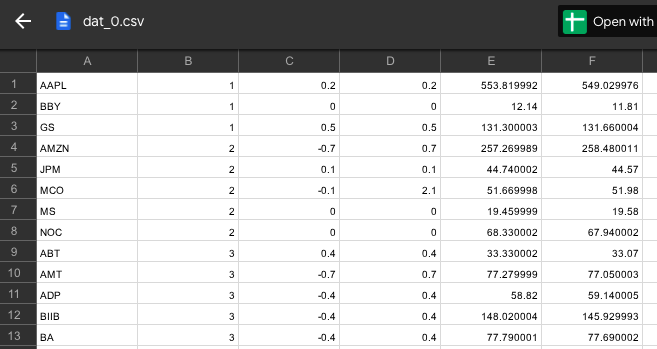
\includegraphics[width=0.5\textwidth]{Sentiment.png}
\end{center}
\\
The Data Produced above is used in our neural network which breaks the data into train and test data to use it the our Google's Tensorflow Model. After Training the model for about 22,000 epochs the test error converges at 0.0094688255
\begin{center}
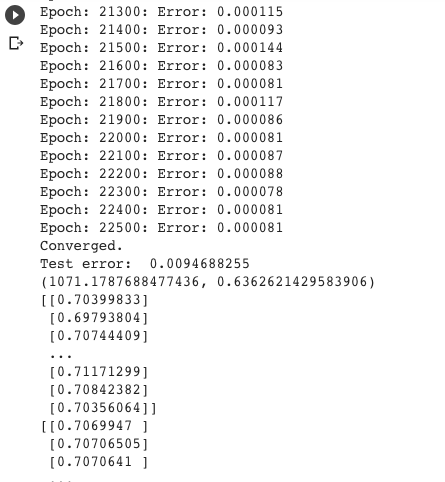
\includegraphics[width=0.5\textwidth]{Accuracy.png}
\end{center}
\begin{center}

\\
The Following is the plot for the error and it's corresponding epochs. Here We observe that while the initial Epochs held the error of about 2 we have reached the saturation point at somewhere at 12000 epochs where it has come down to about 0.009.
\begin{center}
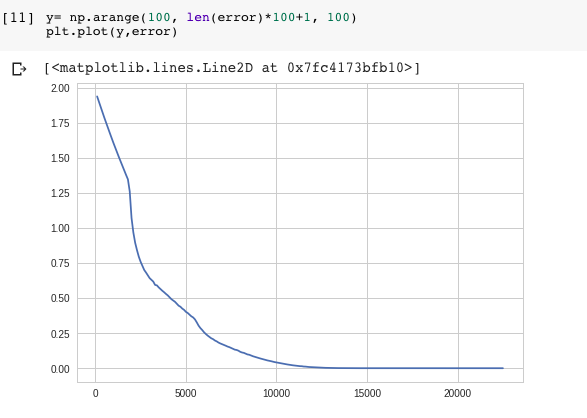
\includegraphics[width=0.5\textwidth]{acc_epochs.png}
\end{center}
\begin{center}
 \ \
 
\end{document} 